\section{Introduction}

\paragraph{Motivation}
In recent years, Neural NNs have had a lot of success in image classification.
This has led to advances in many areas, including computer vision and object recognition.
E.g. advances in a constantly ongoing "ImageNet classification challenge", which were achieved
through new approaches,
rather than increasing NNs number of layers and parameters~\cite{russakovsky2015imagenet,DBLP:journals/corr/abs-1905-11946}.
However, NNs are also vulnerable to adversarial attacks~\cite{ilyas2019adversarial}.
Adversarial attacks are designed to fool neural networks into miss-classifying data.
This can have serious consequences, as it can lead to incorrect results or decisions.
Assuring trust-worthiness of ML classifiers is researches obligation.

\paragraph{Adversarial attack}
Goodfellow defined adversarial attacks as “inputs to machine learning models that an
attacker has intentionally designed to cause the model to make a mistake.”
~\cite{DBLP:journals/corr/abs-1802-08195} \\
In the domain of image classification, adversarial attacks are usually formed by applying a small perturbation (which
is barely noticeable for human viewer) to a naturally occurring image, with the intention of making NN miss-classify.
There are many types of adversarial attacks.
This paper focuses on white-box attacks, where the attacker has full access to the model and its parameters,
namely FGSM.

\paragraph{FGSM}
This method was first introduced by Goodfellow and Jonathon Shlens and Christian Szegedy
~\cite{goodfellow2015explaining}.
It produces adversarial images which make NN miss-classify,
but are still recognisable as of the same class for human viewer.
An example of such images can be seen in~\ref{fig:fig-adv}.
FGSM works by using the gradients of the neural network to create an adversarial pattern.
For an input image,
the method evaluates the signed gradient of the loss function with respect to the input image to create a pattern,
which maximizes the loss.
The pattern is then added pixel wise to the original image.
The new image is called the adversarial image.
The process can be summarised using the following expression:
\begin{equation}
    adv\_x = x + \epsilon \cdot sign(\nabla_x J(\theta, x, y))
\end{equation}
where: \\
$adv_x$ is the resulting image, \\
$x$ is the original image, \\
$\epsilon$ is the intensity of adversarial pattern, \\
$J$ is the loss function, \\
$\theta$ is NNs parameters, \\
$y$ is the original label.
\\
\begin{figure}[h]
    \begin{subfigure}{0.4\textwidth}
        \caption{Tulips 40\% confidence}
        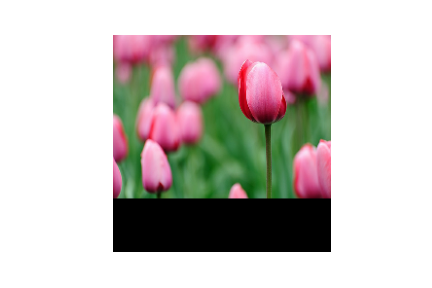
\includegraphics[width=8cm]{images/og_image}
    \end{subfigure}
    \begin{subfigure}{0.4\textwidth}
        \caption{Adversarial pattern for this image}
        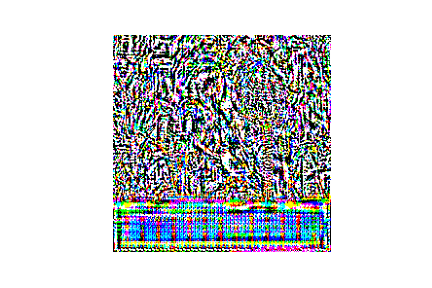
\includegraphics[width=8cm]{images/adv_pattern}
    \end{subfigure}
    \\
    \begin{subfigure}{0.4\textwidth}
        \caption{$\epsilon = 0.01$, Roses 40\% confidence}
        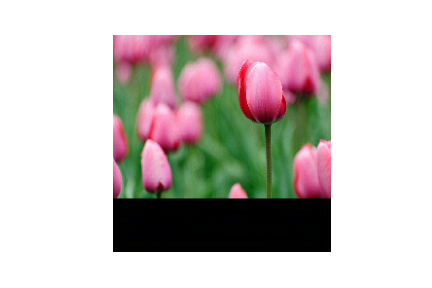
\includegraphics[width=8cm]{images/adv_attack_001}
    \end{subfigure}
    \begin{subfigure}{0.4\textwidth}
        \caption{$\epsilon = 0.1$, Roses 40\% confidence}
        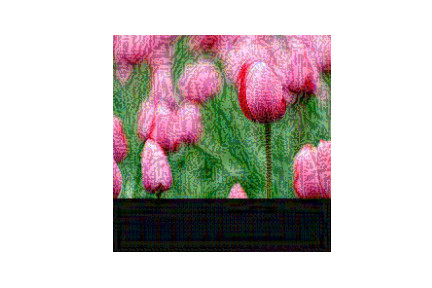
\includegraphics[width=8cm]{images/adv_attack_01}
    \end{subfigure}

    \caption{An example image, adversarial pattern created from it, and adversarial attack with different values of $\epsilon$}
    \label{fig:fig-adv}
\end{figure}



\paragraph{some meanigfull transition} bla bla bla
\\
\\
One should always want to train ML classifier, in such a way, which maximizes generalization.
Naive approach for this would be to provide as much diverse training data as possible.
This approach, however, heavily relies on a collection and labeling of data by humans, which is an extremely time-consuming

\paragraph{Transfer Learning}
Another popular technic aiming to improve ML classifiers accuracy is called Transfer Learning (TL).
TL is a training approach in ML, which focuses on storing knowledge gained while solving one
problem and applying it to a different but related problem.

For example, knowledge gained while learning to recognize cars could apply when trying to recognize trucks.
Concrete for ML engineers this could mean reusing one of the NNs, which performed the best at e.g.
"ImageNet classification challenge", and then fine-tuning it for a concrete downstream task of interest.
This eliminated the need of collecting and labeling more data for concrete classification problem,
however, it still heavily relies on the existence of big labeled datasets.
Not to forget, that while NN reuses the learned features, the NN will also reuse
the biases learned from previous datasets, which makes them once again more dependable on labeling previously done by a human.


\paragraph{Self-Supervised Learning Framework}
In contrast to previously described frameworks, the Self-Supervised Learning framework, requires relatively small amount
of data to produce a big variety of labeled training data.
One of its core features, is that
labeling of new data is not dependent on humans, and can be done in seconds by the ML classifier itself.

E.g. NN applies multiple pre-defined data augmentations to existing data and overwrite the labels by corresponding
pseudo-labels, and then is trained to predict which one was applied.
This allows multiplying the size of
training dataset by a number of pre-defined documentations, and also increasing the diversity of training data a
(the metric to measure this, is out of the scope of this paper).

Normally, after self-supervised learning, similarly to TL fine-tuning would be executed.
These parts of training are called pre-text task (or training) and downstream task (or training) respectively.

\paragraph{Pretext task}
Pretext task is the self-supervised learning task solved to learn visual representations,
with the aim of using the learned representations or model weights obtained in the process, for the downstream task.
More concrete for image-classification, the weights of convolutional layers will be frozen after pre-text training,
with the aim of reusing the features learned, similarly to TL.

It has been shown that pretext tasks can significantly improve NNs accuracy~\cite{kolesnikov2019revisiting}.
It is also believed they contribute to NNs learning of important (as per human agents) features.
This paper focuses on TL, rotation and jigsaw pre-text tasks.


\paragraph{Related wörk}
The adversarial vulnerability phenomenon is widely known, first described by Ian J. Goodfellow~\cite{goodfellow2015explaining}.
It has been the accompanying success of image classification over the last years.
Up to day, there is no clear solution to this problem.
One of the suggested approaches is Adversarial Training~\cite{https://doi.org/10.48550/arxiv.1805.12152},
during which NN is trained to reduce the loss over worst-case adversarial perturbations.
This, however, comes at a cost of decreased standard classification accuracy, not the least this approach is noticeably more time-consuming
There have also been numerous studies~\cite{kolesnikov2019revisiting,DBLP:journals/corr/NorooziF16,DBLP:journals/corr/abs-1912-01991}
on how pretext tasks, and their choice can influence standard classification accuracy.
On the other hand, there were no studies, which investigated the impact of pretext task choice on
adversarial vulnerability. \\
This study was motivated by \st{curiosity} increasing demand in highly accurate robust trust-worthy ML classifiers.



\section{Methods}

\paragraph{Model}
Convolutional networks' architectures for image recognition have evolved quite drastically in recent years,
with numerous options available "out of the box".
A.e.\ Efficient Net (EffNet) delivers impressive accuracy, while being able to scale better than a lot of
previous architectures~\cite{DBLP:journals/corr/abs-1905-11946}.
For this paper, the evaluation was done using it, namely EfficientNetB0~\cite{KerasEffNet}

\paragraph{Rotation pretext task}
A common choice of pretext task could be to produce 4 copies of
a single image by rotating it by {0°, 90°, 180°, 270°} and let a single network predict the rotation which was applied.
Alexander Kolesnikov and Xiaohua Zhai and Lucas Beyer: "Intuitively, a good model should learn to
recognize canonical orientations of objects in natural images" ~\cite{kolesnikov2019revisiting}.
For this papers evaluation, each image from the original dataset was rotated 0°, 90°, 180°,
270° and assigned a new pseudo label from [0, 1, 2, 3] accordingly.
The examples of such images are shown in~\ref{fig:rot-fig}.
All 4 batches of rotated images, as well as pseudo labels were concatenated in new dataset, and shuffled.
Then EffNet was then trained to identify rotation applied, afterwards the convolutional layers were frozen,
and the output layer size was adjusted for the downstream task.

\begin{figure}[h]
    \begin{subfigure}{0.33\textwidth}
        \caption{Label = 0}
        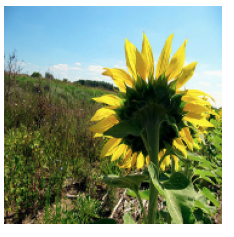
\includegraphics[width=5cm]{images/rot_0}
    \end{subfigure}
    \begin{subfigure}{0.2\textwidth}
        \caption{Label = 1}
        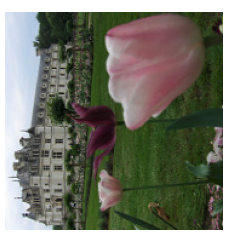
\includegraphics[width=5cm]{images/rot_1}
    \end{subfigure}
    \begin{subfigure}{0.33\textwidth}
        \caption{Label = 2}
        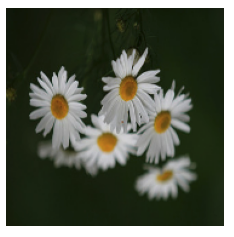
\includegraphics[width=5cm]{images/rot_2}
    \end{subfigure}
    \caption{An example how images used for rotation pretext task could look like}
    \label{fig:rot-fig}
\end{figure}




\paragraph{Jigsaw pretext task}
The task is
to recover relative spatial position of 4 sampled image patches
after a random permutation of these patches was performed
~\cite{kolesnikov2019revisiting}.
All of these patches are concatenated in 'puzzle' image,
which is later sent through same network, which needs to predict a permutation applied.\
A similar approach as described by Mehdi Noroozi and Paolo Favaro~\cite{DBLP:journals/corr/NorooziF16} was adopted.
Random 4 out of 24 possible permutations were chosen for each batch
(number of possible permutation can be obtained from Newtonian binomial $P=\frac{r!}{(r-n)!}$).
For each permutation, each image was cut in 4 equal parts,
afterwards these tiles were permuted as per chosen permutation, and concatenated in 1 (puzzle) image.
An example can be seen in~\ref{fig:jig-fig}.
Similarly, to rotation pseudo labels in [0\ldots23] had been assigned,
NN was trained to identify permutation applied.
Then the weights of convolutional layers were frozen and reused for the downstream task.

\\
\begin{figure}[h]
    \begin{subfigure}{0.33\textwidth}
        \caption{Original image}
        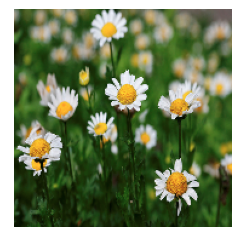
\includegraphics[width=5cm]{images/dandelion}
    \end{subfigure}
    \begin{subfigure}{0.2\textwidth}
        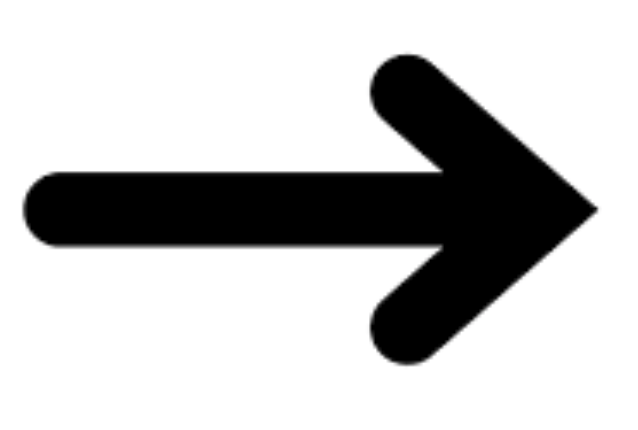
\includegraphics[width=3cm]{images/arrow}
    \end{subfigure}
    \begin{subfigure}{0.33\textwidth}
        \caption{Generated puzzle, label=1}
        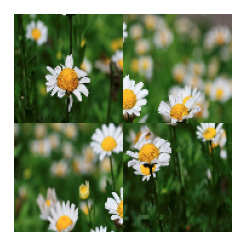
\includegraphics[width=5cm]{images/puzzle}
    \end{subfigure}
    \caption{An example how puzzle for jigsaw pretext task could look like}
    \label{fig:jig-fig}
\end{figure}



For this paper, EffNet was pre-trained on "imagenette"~\cite{ImageNette} dataset for image classification. and then
Imagenette is a subset of 10 easily classified classes from the Imagenet dataset.
Afterwards the NN was fine-tuned for an actual classification task of interest on~\cite{tfflowers}.

\paragraph{Adversarial Images with FGSM}
The implementation of FGSM for this paper was based on \cite{FGSM}.
In order to generate adversarial pattern for each image,
gradient of loss function is evaluated with sign for each image.
Then as per previously described approach,
adversarial pattern was added pixel wise to the original image with $\epsilon = 0.01$.
Resulting adversarial image was then clipped by value, so each channels' value stays in interval [0\ldots255],
as required for RGB color encoding.

\paragraph{Evaluation approach}
In order to evaluate, how including pretext task in the training process influences NNs vulnerability against adversarial attacks,
I have measured miss-classification rate while keeping the intensity of adversarial pattern fixed at $\epsilon = 0.01$.
\\
Following metrics of interest were recorded:

\begin{equation}
    Accuracy_i = \frac{\# \; images \; correctly \; classified_i}{\# \; test \; images_i} \cdot 100 \%
\end{equation} \\
where Accuracy\_i is the accuracy in each evaluation round \\
\# stands for "number".
\begin{equation}
    \overline{Accuracy} = \frac{1}{N}  \sum_{i=1}^{N}{Accuracy_i}
\end{equation}


\begin{equation}
    Miss \; rate_i = \frac{\# images \; miss \; classified_i}{\# \; images \; correctly \; classified_i} \cdot 100 \%
\end{equation}
where Miss rate\_i is the miss rate in each evaluation round.
\begin{equation}
    \overline{Miss \; rate} = \frac{1}{N}  \sum_{i=1}^{N}{Miss \; rate_i}
\end{equation}


The dataset "tf\_flowers"~\cite{tfflowers} was chosen for experiment, 5\% of dataset were reserved for evaluation.
\\
During each evaluation round NN network was pre-trained either with transfer learning, or rotation, or jigsaw.
The number of training epochs was varied in [15, 30, 45, 60] for pretext training, while the number of epochs for downstream
training was fixed at 30.
\\
The reserved for evaluation images were given to NN. The number of correct classifications was recorded.
Then, for each previously correctly classified image FGSM with $\epsilon = 0.01$ was applied.
The number of miss-classifications was recorded afterwards.
